% What is on the Tang Nano 9K: its parts, the documents that describe them, the BL702 bridge,
% USB hosts and devices, and a USB host inside the FPGA. Build with ./build.sh.

\documentclass[11pt,a4paper]{article}

\usepackage{fontspec}
\usepackage[margin=2.5cm]{geometry}
\usepackage{float}
\usepackage{enumitem}
\usepackage{booktabs}
\usepackage{array}
\usepackage{chapter}
\usepackage[colorlinks=true,linkcolor=blue!50!black,urlcolor=blue!50!black]{hyperref}

% Text quoted from a datasheet, in sans, set off from the lesson's own voice.
\newenvironment{datasheet}{\begin{quote}\small\sffamily}{\end{quote}}

\setlength{\parindent}{0pt}
\setlength{\parskip}{0.6em}

\title{What is on the board}
\author{}
\date{}

\begin{document}
\maketitle

\begin{figure}[H]
  \centering
  \begin{tikzpicture}[box/.style={draw, thick, align=center, font=\small},
      part/.style={draw, thick, align=center, font=\footnotesize\sffamily, minimum width=2.3cm, minimum height=0.7cm},
      lbl/.style={font=\scriptsize\sffamily, above, inner sep=1.5pt}]
    \draw[black!45, rounded corners=3pt] (-1.4,-2.6) rectangle (12.3,2.6);
    \node[font=\small\bfseries, anchor=south west] at (-1.4,-2.6) {\name{Tang Nano 9K}};
    \node[box, minimum width=1.3cm, minimum height=1.2cm] (usb) at (-0.4,0) {\sffamily USB-C};
    \node[box, minimum width=2.2cm, minimum height=2.2cm] (bl) at (2.6,0) {\name{BL702}\\[0.2em]\scriptsize USB-JTAG and\\\scriptsize USB-UART\\\scriptsize bridge};
    \node[box, minimum width=2.6cm, minimum height=3.6cm] (fpga) at (6.8,0) {\name{GW1NR-9}\\[0.2em]\scriptsize FPGA, with\\\scriptsize PSRAM inside};
    \draw[<->] (usb) -- node[lbl] {D+, D$-$} (bl);
    \draw[->] ([yshift=0.6cm]bl.east) -- node[lbl] {JTAG} ([yshift=0.6cm]bl.east -| fpga.west);
    \draw[<->] ([yshift=-0.6cm]bl.east) -- node[lbl] {UART} ([yshift=-0.6cm]bl.east -| fpga.west);
    \pic at (4.4,-1.4) {crystal};
    \node[font=\scriptsize, below] at (4.4,-1.8) {27\,MHz};
    \draw[->] (4.7,-1.4) -- (5.5,-1.4);
    \foreach \t [count=\i from 0] in {SPI flash, HDMI, RGB LCD, SPI LCD, microSD} {
      \node[part] (p\i) at (10.5,1.6-0.8*\i) {\t};
      \draw[<->] (8.1,1.6-0.8*\i) -- (p\i);
    }
    \node[font=\scriptsize, align=left, anchor=north west] at (5.5,2.45) {6 LEDs, 2 buttons, 48 header pins};
  \end{tikzpicture}
\end{figure}

The \name{Tang Nano 9K} carries two programmable chips, not one. The FPGA runs the designs. Beside it, a small RISC-V microcontroller, the \name{BL702}, runs a program of its own and turns the board’s USB-C port into two things the Mac can use. One is a JTAG port that loads designs into the FPGA, and the other is a serial line to it. This lesson explains every chip on the board, what it does there, and what a design can do with it. It then says which document describes each part, follows the \name{BL702}’s wires, says what it could still do, and asks what it would take to plug a USB keyboard into the board.

\section*{Reading first}

The board’s own datasheet has four numbered pages, and most of what the board is lives in the other documents. Read them in this order:
\begin{enumerate}
  \item The board’s datasheet~\cite{tnds}, pp.~1 and~3. Page~1 is the hardware table, whose \emph{Debugger} row names the \name{BL702}. Page~3 is the photo with each part labelled.
  \item The board’s schematic~\cite{schematic}, all five sheets. The \name{BL702} and the USB-C connector are on PDF page~4, which is sheet 5 of 5.
  \item Horowitz and Hill~\cite{aoe}, §14.7, \emph{Serial buses and data links}, pp.~1032--1043. Within it, §14.7.4, \emph{JTAG}, is on p.~1036, §14.7.8, \emph{Asynchronous serial}, on p.~1038, and §14.7.13, \emph{USB}, on p.~1042.
  \item Harris and Harris~\cite{ddca}, §9.3.5, \emph{Serial I/O}, pp.~542.e14--542.e29. It covers SPI first and the UART from p.~542.e23, with a UART connected to a PC through a USB adapter.
  \item \emph{USB in a NutShell}~\cite{nutshell}, chapters 1 and 2. They explain hosts and devices, the speeds, and how a device announces its speed with a pull-up resistor.
  \item The \name{BL702}’s datasheet~\cite{blds}: the feature list on PDF page~2, §2.7, \emph{Boot}, and §2.10.9, \emph{USB2.0 (Full Speed)}.
\end{enumerate}

\section*{The parts, one by one}

\begin{figure}[H]
  \centering
  \begin{tikzpicture}[x=0.538bp, y=-0.538bp, ring/.style={draw=red, line width=0.8pt}]
    \node[anchor=north west, inner sep=0] at (0,0)
      {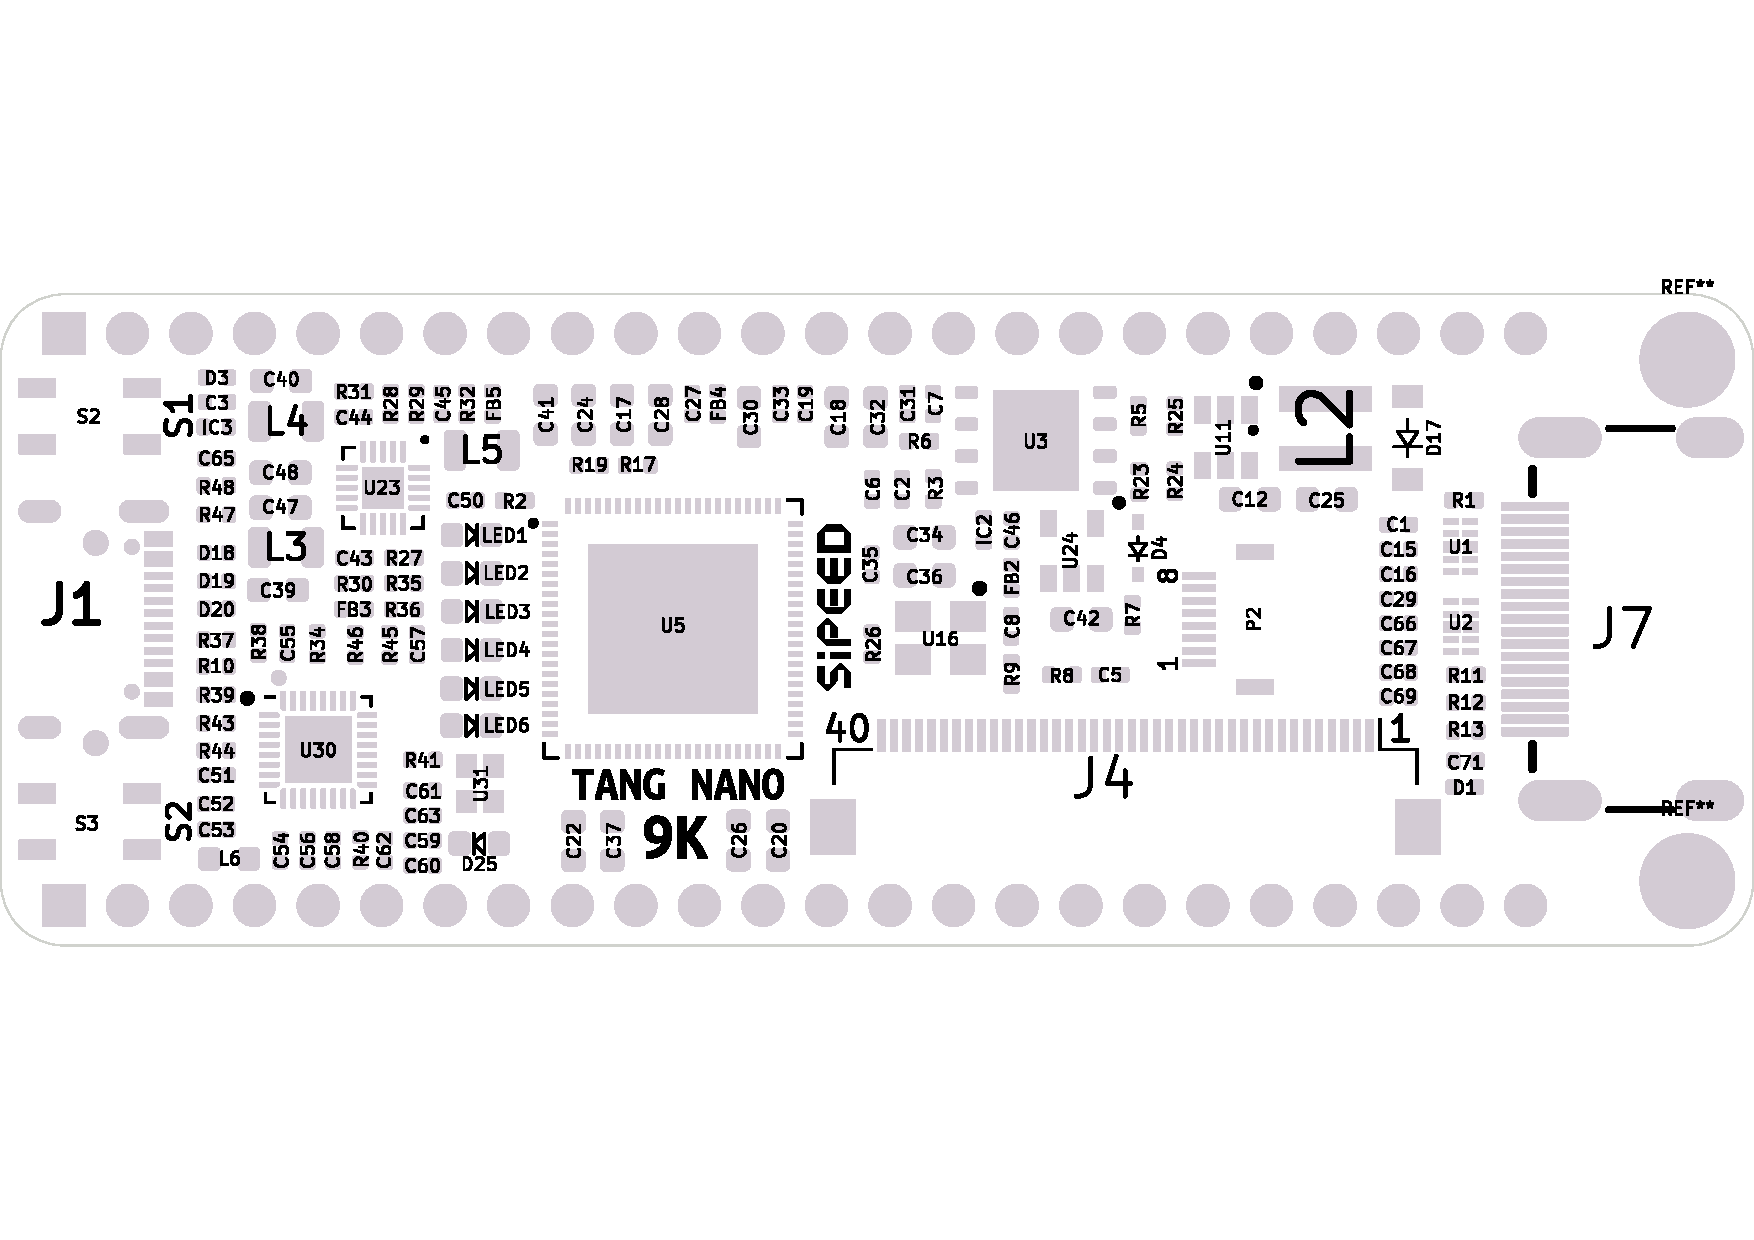
\includegraphics[trim=0 138.32 0 138, clip, scale=0.538]{assets/tang-nano-9k-top.pdf}};
    \draw[ring] (322.6,162) circle (52);
    \foreach \x/\y/\r in {182.4/96.2/24, 152.6/222/30, 230.4/236.4/16, 451.2/168.2/24, 496.8/73.2/26,
                          512.6/126/18, 586.6/72.2/18, 701.8/125/14, 701.8/161/14}
      \draw[ring] (\x,\y) circle (\r);
  \end{tikzpicture}
  \caption{The top of the board, with its chips circled~\cite{topview}. Table~\ref{tab:parts} names them, and the sections below describe them.\label{fig:top}}
\end{figure}

The board has nine chips, a few connectors, and about a hundred small resistors, capacitors, and diodes~\cite{ibom}. Each part is named by its designator, as in the schematic, so that it can be found in the figure and in the schematic. The sections below come in three groups. First come the chips that make the board run, then the connectors that a design can drive, and last the buttons, the LEDs, the header pins, and the small parts. Table~\ref{tab:parts} lists them in the same order.

\begin{table}[H]
  \centering
  \small
  \begin{tabular}{rlll}
    \toprule
    & Part & What it is & What it does \\
    \midrule
    1 & \name{U5} & \name{GW1NR-9} FPGA & runs the designs \\
    2 & \name{U16} & 27\,MHz oscillator & clocks the FPGA \\
    3 & \name{U3} & SPI flash, 4\,MB & stores data for a design \\
    4 & \name{U30}, \name{U31} & \name{BL702} and its crystal & joins USB to the FPGA’s JTAG and UART \\
    5 & \name{U23}, \name{U24} & step-down converters, regulator & make 3.3, 1.8, and 1.2\,V \\
    6 & \name{J4}, \name{U11} & RGB LCD connector, backlight & drive a parallel screen \\
    7 & \name{J7}, \name{U1}, \name{U2} & HDMI connector, protection & send video to a monitor \\
    8 & \name{P2} & SPI LCD connector & drives a small screen \\
    9 & \name{J3} & microSD slot, underneath & holds files, such as disk images \\
    10 & \name{S1}, \name{S2}, \name{LED1}--\name{LED6} & buttons and LEDs & 1.8\,V inputs and outputs \\
    11 & \name{J5}, \name{J6} & header pins & bring 48 pins to the breadboard \\
    12 & --- & resistors, capacitors, diodes & protect and filter \\
    \bottomrule
  \end{tabular}
  \caption{The board’s parts, in the order of the sections below.}\label{tab:parts}
\end{table}

\subsection*{The FPGA, \name{U5}}

The \name{GW1NR-9} is the chip that runs the designs. It has 8640 four-input lookup tables (LUTs) and 6480 flip-flops for logic, 26 blocks of block RAM holding 468\,Kbit in all, twenty 18-by-18-bit multipliers, and two PLLs, which multiply the clock~\cite[p.~1]{tnds}. Its package holds two more chips. One is 64\,Mbit of PSRAM, a memory that refreshes itself, which a design reaches through a controller. The other is the flash that keeps the design across power cycles, with 608\,Kbit more of user flash beside it~\cite[p.~1]{tnds}.

For the Altair, the block RAM holds 58.5\,KB, which is almost the 64\,KB an 8080 can address, and the PSRAM holds all of it with room to spare.

\subsection*{The clock, \name{U16}}

\name{U16} is a 27\,MHz crystal oscillator, which is a quartz crystal and the amplifier that keeps it ringing, sealed in one four-pin package. It runs from 3.3\,V, and its output reaches FPGA pin 52 through a 22\,$\Omega$ resistor~\cite[p.~2]{schematic}. Every design starts from this clock. The PLLs inside the FPGA turn it into other frequencies, such as the pixel clock of a screen.

\subsection*{The SPI flash, \name{U3}}

\name{U3} is a \name{PUYA P25Q32U}, a 32\,Mbit (4\,MB) flash memory with a serial (SPI) interface. It is wired to FPGA pins 59 to 62, which are the clock, chip select, data out, and data in of the FPGA’s SPI port~\cite[p.~2]{schematic}. It is separate from the flash inside the FPGA, which holds the design. A design can read and write it as storage, for instance to keep BASIC tapes or CP/M disk images.

\subsection*{The USB bridge, \name{U30} and \name{U31}}

\name{U30} is the \name{BL702}, the microcontroller that joins the USB-C port to the FPGA, and \name{U31} is its 32\,MHz crystal. The orange LED \name{D25}, next to \name{U31}, shows the bridge’s state. The sections after this one follow the bridge in detail.

\subsection*{The power supply, \name{U23} and \name{U24}}

The board takes 5\,V from the USB-C port and makes four lower voltages from it. \name{U23}, a \name{TMI7003C}, holds three step-down converters, also called buck converters. Each one switches the 5\,V on and off very fast and smooths the result with an inductor, \name{L3} to \name{L5}, so little power turns into heat. Two resistors set each output to $0.6 \times (1 + R_a/R_b)$\,V. With 680\,k$\Omega$ and 150\,k$\Omega$, two of the outputs are 3.3\,V. One feeds the other chips and the header’s 3.3\,V pin, and the other feeds the FPGA’s I/O banks 0, 1, and 2. With 300\,k$\Omega$ and 150\,k$\Omega$, the third output is 1.8\,V, which feeds bank 3~\cite[p.~3]{schematic}. Each channel delivers up to 1.5\,A~\cite{tmi}.

\name{U24}, an \name{ME6211C12}, is a linear regulator that makes 1.2\,V from 3.3\,V for the FPGA’s core~\cite[p.~3]{schematic}. A linear regulator turns the difference in voltage into heat, which is acceptable for the core’s small current.

The banks are why some FPGA pins work at 1.8\,V. Every pin in bank 3 swings between 0 and 1.8\,V, and that bank holds the buttons, the LEDs, and the header pins \name{R2} to \name{R9}.

\subsection*{The RGB LCD and its backlight, \name{J4} and \name{U11}}

\name{J4} is a 40-pin flat-cable connector for a parallel RGB screen, such as Sipeed’s 5-inch LCD. The FPGA sends each pixel’s red, green, and blue bits on separate pins, together with a pixel clock and sync signals.

The screen’s backlight is a string of LEDs in series, which needs much more than 5\,V. \name{U11}, an \name{LP3320}, is a boost converter that raises the 5\,V to whatever the string needs, with the inductor \name{L2}, the diode \name{D17}, and a capacitor rated for 50\,V, \name{C25}. The 13\,$\Omega$ resistor \name{R25} sets the current through the LEDs, and FPGA pin 86 switches the converter on and off, so a design can dim the backlight by pulsing that pin~\cite[p.~2]{schematic}.

Eight of the LCD’s colour pins are the same FPGA pins as the HDMI lines. Their names in the schematic carry both roles, such as \name{PIN75\_RGB\_R3/HDMI\_D2\_P}~\cite[p.~2]{schematic}. A design therefore drives either the LCD or the HDMI output.

\subsection*{The HDMI connector, \name{J7}, with \name{U1} and \name{U2}}

\name{J7} takes HDMI video. The FPGA drives its four differential pairs, three for colour and one for the clock, straight from its pins. \name{U1} and \name{U2} are \name{RCLAMP0524P}s, which protect those lines from static electricity, and eight 49.9\,$\Omega$ resistors on the back of the board sit on the same lines~\cite[p.~5]{schematic}. A design can show the Altair’s terminal on any monitor or projector this way.

\subsection*{The SPI LCD connector, \name{P2}}

\name{P2} is an 8-pin flat-cable connector for the small 1.14-inch screen, which takes commands and pixels over SPI on FPGA pins 76 and 77, with chip select on pin 48~\cite[p.~2]{schematic}. Its backlight runs from 3.3\,V through the 5.1\,$\Omega$ resistor \name{R7}, and its supply through the diode \name{D4}.

\subsection*{The microSD slot, \name{J3}}

The slot sits on the back of the board. The card speaks SPI on FPGA pins 36 to 39, and diodes protect each line from static~\cite[p.~2]{schematic}. A design can read and write the card block by block, which is how the Altair could keep its floppy disks.

\subsection*{Buttons and LEDs}

The buttons \name{S1} and \name{S2} are on FPGA pins 4 and 3. Each has a 10\,k$\Omega$ resistor to 1.8\,V, so it reads high at rest and low while pressed, and a 100\,nF capacitor that smooths its bounce~\cite[p.~2]{schematic}. The six orange LEDs, \name{LED1} to \name{LED6}, are on pins 10, 11, 13, 14, 15, and 16, and each lights while its pin is low.

\subsection*{The header pins, \name{J5} and \name{J6}}

The two rows of 24 pins bring FPGA pins to the breadboard. \name{J6}, the right-hand row, also carries power. \name{R18} is 5\,V, \name{R23} is GND, and \name{R24} is 3.3\,V~\cite[p.~2]{schematic}. Many header pins are shared with the connectors. \name{L1} to \name{L4} are the microSD lines, \name{L11} to \name{L22} are LCD lines, \name{L23}, \name{L24}, and \name{R12} to \name{R17} are HDMI lines, and \name{R10}, \name{R11}, \name{R19}, and \name{R20} are lines of the small SPI screen, so a pin wired on the breadboard must stay free of whatever is plugged into its connector.

\subsection*{The small parts}

The rest are support parts. Small ESD diodes protect the buttons, the microSD lines, and the USB lines from static electricity. Ferrite beads filter the supply rails, and 22\,$\Omega$ resistors in series with fast signals tame their edges. Dozens of capacitors, 100\,nF and 10\,µF most of all, sit next to the chips and supply the short bursts of current that each clock edge draws.

\section*{The documents}

Each document answers a different question, and they nest. The board’s datasheet says what is on the board. The schematic says how each part is wired. The chips’ own documents say what each part can do.

\begin{description}[style=nextline, leftmargin=1.5em]
  \item[Board datasheet~\cite{tnds}, 6 PDF pages] Sipeed’s summary: the hardware table, the working conditions, the labelled photo, and the board’s size.
  \item[Schematic~\cite{schematic}, 5 sheets] Every part, every wire, and every resistor value. It is the board’s real documentation, and it answers which FPGA pin goes where, which pins reach a header, and which bank runs at 1.8\,V.
  \item[Top designator drawing~\cite{topview}] Where each part and header pin sits on the board.
  \item[GW1NR datasheet~\cite{gw1nr}, 76 pages] Gowin’s description of the FPGA family: logic, memories, I/O standards, and the electrical limits of the pins.
  \item[Gowin user guides~\cite{gowin}] One guide per topic, such as the clocks and the PLLs (UG286) and the programmable I/O (UG289), which sets a pin’s drive strength and its pull-up or pull-down.
  \item[\name{BL702} datasheet~\cite{blds}, 54 pages] Bouffalo Lab’s summary of the microcontroller: its features, its pins, and its electrical limits.
  \item[\name{BL702} reference manual~\cite{blrm}, 339 pages] Every register of every peripheral, for whoever writes the \name{BL702}’s firmware. Its USB chapter, chapter~18, starts on PDF page~292.
\end{description}

\section*{The bridge is a computer}

The \name{BL702} is a complete microcontroller. Its CPU is a 32-bit RISC-V core at up to 144\,MHz, with 132\,KB of RAM, 512\,KB of flash on the chip, and 192\,KB of ROM~\cite[p.~2]{blds}. It has a 2.4\,GHz radio for Bluetooth Low Energy 5.0 and Zigbee 3.0, and a USB 2.0 full-speed device interface, 12\,Mbit/s~\cite[p.~2]{blds}. On this board, it runs one program, which makes it look to the Mac like an FTDI \name{FT2232D}, a common USB chip with two channels~\cite{rvdebugger}. Channel A drives the JTAG lines and channel B is the UART, so the Mac lists two serial ports. \name{openFPGALoader} talks to it as it would to the FTDI chip~\cite{ofl}.

The datasheet’s feature list~\cite[PDF p.~2]{blds} opens with the radio and lists the USB interface among the peripherals:
\begin{datasheet}
Wireless: 2.4 GHz RF transceiver; Bluetooth® Specification v5.0; Bluetooth® Low Energy 1Mbps and 2Mbps; Bluetooth® Long Range Coded 500Kbps and 125Kbps; Zigbee 3.0, Base Device Behavior, Core Stack R21, Green Power; IEEE 802.15.4 MAC/PHY; Support BLE/zigbee coexistence; Integrated balun, PA/LNA.

Peripheral: USB2.0 FS (Full-Speed) device interface.
\end{datasheet}

\begin{figure}[H]
  \centering
  \resizebox{\linewidth}{!}{%
  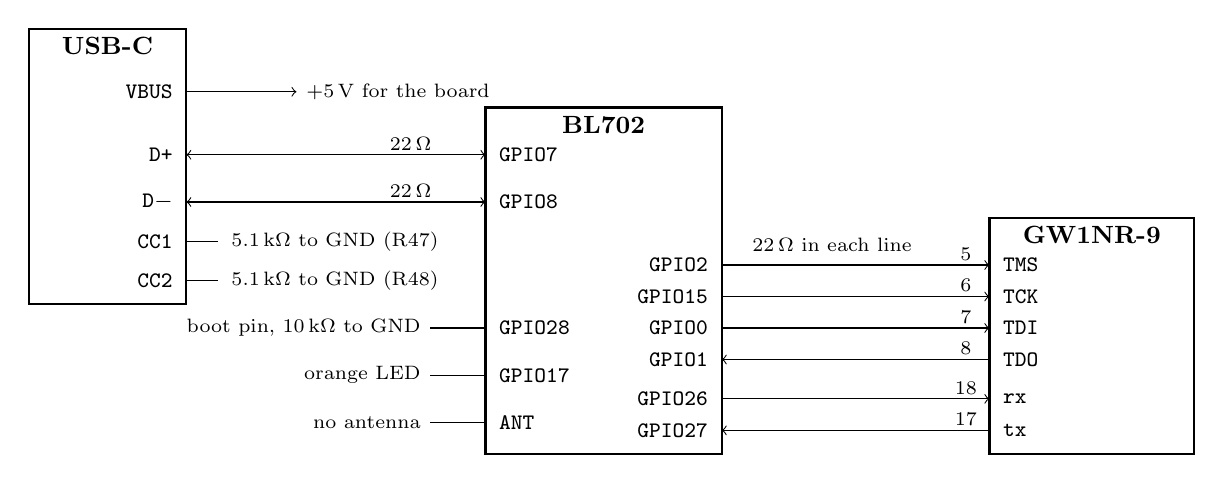
\begin{tikzpicture}[
      port/.style={font=\footnotesize\ttfamily},
      pin/.style={font=\scriptsize, above, inner sep=1.5pt},
      title/.style={font=\small\bfseries, inner sep=3pt}]
    % USB-C connector
    \draw[thick] (-0.8,-1.1) rectangle (1.2,2.4);
    \node[title, anchor=north] at (0.2,2.4) {USB-C};
    \foreach \y/\l in {1.6/VBUS, 0.8/D+, 0.2/D$-$, -0.3/CC1, -0.8/CC2} \node[port, anchor=east] at (1.15,\y) {\l};
    % CC pull-downs
    \foreach \y/\r in {-0.3/R47, -0.8/R48} {
      \draw (1.2,\y) -- (1.6,\y);
      \node[font=\scriptsize, anchor=west] at (1.65,\y) {5.1\,k$\Omega$ to GND (\r)};
    }
    \draw[->] (1.2,1.6) -- (2.6,1.6) node[right, font=\scriptsize] {+5\,V for the board};
    % BL702
    \draw[thick] (5.0,-3.0) rectangle (8.0,1.4);
    \node[title, anchor=north] at (6.5,1.4) {\name{BL702}};
    \foreach \y/\l in {0.8/GPIO7, 0.2/GPIO8} \node[port, anchor=west] at (5.05,\y) {\l};
    \draw[<->] (1.2,0.8) -- node[pin, pos=0.75] {22\,$\Omega$} (5.0,0.8);
    \draw[<->] (1.2,0.2) -- node[pin, pos=0.75] {22\,$\Omega$} (5.0,0.2);
    \foreach \y/\l in {-0.6/GPIO2, -1.0/GPIO15, -1.4/GPIO0, -1.8/GPIO1, -2.3/GPIO26, -2.7/GPIO27} \node[port, anchor=east] at (7.95,\y) {\l};
    \foreach \y/\l in {-1.4/GPIO28, -2.0/GPIO17, -2.6/ANT} \node[port, anchor=west] at (5.05,\y) {\l};
    \draw (5.0,-1.4) -- (4.3,-1.4) node[left, font=\scriptsize, align=right] {boot pin, 10\,k$\Omega$ to GND};
    \draw (5.0,-2.0) -- (4.3,-2.0) node[left, font=\scriptsize] {orange LED};
    \draw (5.0,-2.6) -- (4.3,-2.6) node[left, font=\scriptsize] {no antenna};
    % FPGA
    \draw[thick] (11.4,-3.0) rectangle (14.0,0.0);
    \node[title, anchor=north] at (12.7,0.0) {\name{GW1NR-9}};
    \foreach \y/\l in {-0.6/TMS, -1.0/TCK, -1.4/TDI, -1.8/TDO, -2.3/rx, -2.7/tx} \node[port, anchor=west] at (11.45,\y) {\l};
    \foreach \y/\n/\d in {-0.6/5/->, -1.0/6/->, -1.4/7/->, -1.8/8/<-, -2.3/18/->, -2.7/17/<-} {
      \draw[\d] (8.0,\y) -- (11.4,\y);
      \node[pin] at (11.1,\y) {\n};
    }
    \node[font=\scriptsize, above] at (9.4,-0.55) {22\,$\Omega$ in each line};
  \end{tikzpicture}}
  \caption{The \name{BL702}’s wiring on the \name{Tang Nano 9K}, from sheet 5 of the schematic~\cite[p.~4]{schematic}. The numbers at the FPGA’s edge are its pin numbers. TMS is test mode select, TCK test clock, TDI test data in, and TDO test data out. D+ and D$-$ are USB’s two data lines, and CC1 and CC2 are USB-C’s configuration channels.}
\end{figure}

Two links join the \name{BL702} to the FPGA, and both are serial. The four JTAG lines reach the FPGA’s dedicated JTAG pins, 5 to 8, which load and erase its designs. The UART’s two lines reach ordinary FPGA pins, 17 and 18, where a design can send and receive bytes. The UART is the only path a running design has to the \name{BL702}. Even with new firmware, the \name{BL702} would talk to the FPGA through those two wires.

The radio is unusable here. The chip’s RF pin, \name{ANT}, ends in a net label that appears nowhere else in the schematic, so the board has no antenna and no matching circuit~\cite[p.~4]{schematic}.

\section*{Host and device}

USB is not symmetric. One end is the \emph{host}, which supplies the 5\,V on VBUS and starts every transfer; a PC is a host. The other end is a \emph{device}, which only answers; a keyboard, a mouse, and a gamepad are devices~\cite{nutshell}. A keyboard plugged into the board would need the board to be the host.

The \name{Tang Nano 9K} is a device, for two reasons. The first is the connector. Each of its CC pins has a 5.1\,k$\Omega$ resistor to GND, which tells the other end that this port receives power, and VBUS comes in to become the board’s +5\,V~\cite[p.~4]{schematic}. The second reason is decisive. The \name{BL702}’s USB controller is a device controller only, ‘compliant with full-speed USB device standards’~\cite[§2.10.9]{blds}, and its reference manual lists ‘full speed device-mode’ and no host mode~\cite[ch.~18]{blrm}. A different connector, or new firmware, leaves the \name{BL702} a device.

The datasheet’s section on the controller~\cite[§2.10.9]{blds} describes a device in every line:
\begin{datasheet}
The chip embeds a full-speed USB compatible device controller with the following features: compliant with full-speed USB device standards; has 8 endpoints, each with a 64-byte deep FIFO; all endpoints except endpoint 0 support interrupt/bulk/isochronous transfers; with standby/resume function; USB dedicated 48MHz clock directly generated by internal main PLL.
\end{datasheet}

\section*{Changing the bridge’s firmware}

The \name{BL702}’s firmware is open source. Sipeed’s \name{RV-Debugger-BL702}~\cite{rvdebugger} is the original, written for Sipeed’s stand-alone debugger, and it builds two programs, \name{usb2uartjtag} and \name{usb2dualuart}. The fork \name{Debugger\_for\_TANG\_NANO-9K}~\cite{tn9kfork} adapts it to this board.

Rewriting this firmware puts the FPGA at risk. The \name{BL702} is the only path from the USB-C port to the FPGA’s JTAG pins, so a firmware that does not run leaves the FPGA with whatever its flash already holds, and nothing on the Mac can reach it. The way back is in the chip’s ROM, which can boot from UART, USB, or flash~\cite[§2.7]{blds}. Its boot pin is \name{GPIO28}~\cite[PDF p.~36]{blds}, held low by a 10\,k$\Omega$ resistor on this board~\cite[p.~4]{schematic}. With two test points shorted to pull it high at power-up, the ROM starts instead of the firmware and shows up on the Mac as a USB serial port, through which \name{bflb\_mcu\_tool} writes a new firmware~\cite{tn9kfork}.

The datasheet gives the boot options in §2.7~\cite{blds} and the boot pin in a footnote to its pin table~\cite[PDF p.~36]{blds}:
\begin{datasheet}
BL702/BL704/BL706 supports multiple boot options: UART, USB, and Flash.

BL706C-22-Q2I bootstrap pin: GPIO31, other BL70x bootstrap pin: GPIO28.
\end{datasheet}
The chip on this board is a \name{BL702}, so its boot pin is \name{GPIO28}.

\section*{What the bridge could still do}

New firmware turns the \name{BL702} into a small computer placed between the Mac’s USB and the FPGA’s UART. Its 512\,KB of flash and 132\,KB of RAM can hold and process data, and the wiring allows three uses.

The first is a paper-tape reader. The Altair loaded BASIC from paper tape through its serial line. The firmware could keep a tape image in its flash and play it into the UART when asked, so that BASIC loads with no Mac attached. The 4K BASIC tape holds about 4\,KB, so the flash has room for many tapes.

The second is a different USB device on the Mac. The controller has eight endpoints, which are the separate channels a USB device offers the host, so the firmware can present the board as a USB disk, a MIDI instrument, or several serial ports at once.

The third is a second UART to the FPGA. Sipeed’s \name{usb2dualuart} firmware shows the Mac two serial ports. Port B sends on \name{GPIO26} and receives on \name{GPIO27}, which is the existing link to FPGA pins 18 and 17. Port A sends on \name{GPIO15} and receives on \name{GPIO0}~\cite[\name{firmware/app/usb2dualuart/dev\_cfg.h}]{tn9kfork}. On this board those two pins are the TCK and TDI lines, which reach FPGA pins 6 and 7, so port A runs over the JTAG wires. Two things follow. The \name{BL702} no longer speaks JTAG, so the Mac cannot load designs while this firmware runs. The FPGA’s design must also use pins 6 and 7 as ordinary pins, which Gowin allows with the option \emph{Use JTAG as regular IO} in its \emph{Dual-Purpose Pin} settings~\cite[PDF p.~43]{sug100}. While such a design runs, those pins are not JTAG.

Each of these uses replaces the firmware that loads designs, unless the new firmware keeps its JTAG half, as \name{usb2uartjtag} does. Data between the \name{BL702} and a running design travel at the speed of a serial line, so the \name{BL702} suits jobs that pass bytes, such as tapes and terminals.

\section*{A USB host inside the FPGA}

The host can live in the FPGA instead, on two header pins. Hiromichi Kitahara (hi631) connected a USB gamepad to an NES running on a \name{Tang Nano 9K} this way~\cite{hi631}. A USB-A socket takes its D+ and D$-$ lines straight to two FPGA pins, and the host’s pull-down resistors are the FPGA’s internal ones. The host is a small processor in Verilog, \name{ukp}, which runs a short program from its own ROM. It comes from an earlier project that built a PC-8001 in an FPGA~\cite{hi631}.

The host speaks USB at low speed only, 1.5\,Mbit/s. Most keyboards and mice, and simple gamepads, use low speed, and a device announces it with a 1.5\,k$\Omega$ pull-up on D$-$, where a full-speed device pulls up D+~\cite{nutshell}. The article tried the faster speed, measured a delay on the FPGA’s pins that could not be ignored, and stayed at low speed~\cite{hi631}.

nand2mario turned the same design into a reusable core, \name{usb\_hid\_host}, for keyboards, mice, and gamepads~\cite{hidhost}. It needs no CPU and uses fewer than 300 LUTs, fewer than 250 registers, and one block RAM, against the FPGA’s 8640 LUTs and 26 block RAMs~\cite[p.~1]{tnds}. Its examples are for the \name{Tang Nano 20K} and Lattice boards, and its credits name hi631’s \name{Tang Nano 9K} project as its base.

\begin{figure}[H]
  \centering
  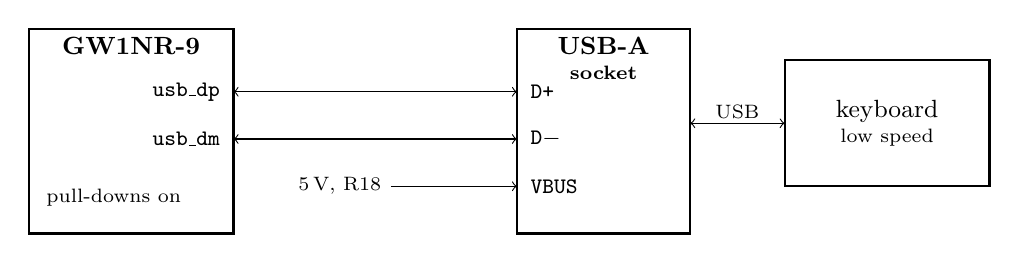
\begin{tikzpicture}[port/.style={font=\footnotesize\ttfamily}, pin/.style={font=\scriptsize, above, inner sep=1.5pt},
      title/.style={font=\small\bfseries, inner sep=3pt}]
    \draw[thick] (0,-1.6) rectangle (2.6,1.0);
    \node[title, anchor=north] at (1.3,1.0) {\name{GW1NR-9}};
    \foreach \y/\l in {0.2/usb\_dp, -0.4/usb\_dm} \node[port, anchor=east] at (2.55,\y) {\l};
    \node[font=\scriptsize, align=left, anchor=west] at (0.1,-1.15) {pull-downs on};
    \draw[thick] (6.2,-1.6) rectangle (8.4,1.0);
    \node[title, anchor=north, align=center] at (7.3,1.0) {USB-A\\[-0.2em]\scriptsize socket};
    \foreach \y/\l in {0.2/D+, -0.4/D$-$, -1.0/VBUS} \node[port, anchor=west] at (6.25,\y) {\l};
    \draw[<->] (2.6,0.2) -- (6.2,0.2);
    \draw[<->] (2.6,-0.4) -- (6.2,-0.4);
    \draw[->] (4.6,-1.0) node[left, font=\scriptsize] {5\,V, \name{R18}} -- (6.2,-1.0);
    \draw[thick] (9.6,-1.0) rectangle (12.2,0.6);
    \node[align=center, font=\small] at (10.9,-0.2) {keyboard\\[-0.2em]\scriptsize low speed};
    \draw[<->] (8.4,-0.2) -- node[pin] {USB} (9.6,-0.2);
  \end{tikzpicture}
  \caption{A USB host in the FPGA. Two FPGA pins in a 3.3\,V bank carry D+ and D$-$, with the FPGA’s internal pull-downs turned on, and the header’s 5\,V pin, \name{R18}~\cite[p.~2]{schematic}, powers the keyboard. The keyboard’s own 1.5\,k$\Omega$ pull-up on D$-$ tells the host it is a low-speed device. The pin names are this sketch’s own.}
\end{figure}

For the Altair, this is the path to a stand-alone machine. A USB keyboard on the FPGA, and the LCD on its connector, would replace the Mac’s terminal, while the USB-C port keeps the serial line for loading paper tapes.

\raggedright
\begin{thebibliography}{RVDBG}
\bibitem[TNDS]{tnds} Sipeed, \textit{Sipeed Tang Nano 9K datasheet}, v1.0, 2021; \name{Sipeed\_Tang\_nano\_9K\_Datasheet\_ENV1.0.pdf} in the books, \name{Tang Nano 9K}.
\bibitem[TN9K]{schematic} Sipeed, \textit{Tang Nano 9K schematic}, \name{Tang\_Nano\_9k\_3672\_Schematic.pdf}, \url{https://dl.sipeed.com/shareURL/TANG/Nano%209K/2_Schematic}; in the books, \name{Tang Nano 9K}.
\bibitem[Top]{topview} Sipeed, \textit{Tang Nano 9K top designator drawing}, \name{Tang\_Nano\_9K\_3672\_Top\_Designator\_Drawing.pdf}; in the repo as \name{docs/assets/tang-nano-9k-top.pdf}.
\bibitem[iBOM]{ibom} Sipeed, \textit{Tang Nano 9K interactive bill of materials}, \name{Tang\_Nano\_9K\_3672\_ibom.html}; in the books, \name{Tang Nano 9K}.
\bibitem[TMI]{tmi} TMI, \textit{TMI7003C datasheet}, \name{tmi7003c.pdf} in the project’s local folder.
\bibitem[GW1NR]{gw1nr} Gowin, \textit{GW1NR series of FPGA products: data sheet}, DS117-3.1E, 2024; \name{GW1NR.pdf} in the books, \name{Tang Nano 9K}.
\bibitem[SUG100]{sug100} Gowin, \textit{Gowin software user guide}, SUG100-2.6E; in the books, \name{Tang Nano 9K/PackAll-en}.
\bibitem[Gowin]{gowin} Gowin, user guides UG286 (clocks) and UG289 (programmable I/O), among others; in the books, \name{Tang Nano 9K/PackAll-en}.
\bibitem[BLDS]{blds} Bouffalo Lab, \textit{BL702/704/706 datasheet}, v2.6, 2022, \url{https://github.com/bouffalolab/bl_docs/tree/main/BL702_DS/en}; in the books, \name{Tang Nano 9K/BL702}.
\bibitem[BLRM]{blrm} Bouffalo Lab, \textit{BL702/BL704/BL706 reference manual}, v1.2, 2023, \url{https://github.com/bouffalolab/bl_docs/tree/main/BL702_RM/en}; in the books, \name{Tang Nano 9K/BL702}.
\bibitem[RVDBG]{rvdebugger} Sipeed, \textit{RV-Debugger-BL702}, \url{https://github.com/sipeed/RV-Debugger-BL702}.
\bibitem[Fork]{tn9kfork} Sergey Koshkin, \textit{Debugger\_for\_TANG\_NANO-9K}, a fork of \name{RV-Debugger-BL702}, \url{https://github.com/koshkin-sergey/Debugger_for_TANG_NANO-9K}.
\bibitem[OFL]{ofl} \textit{openFPGALoader: cables}, \url{https://trabucayre.github.io/openFPGALoader/compatibility/cable.html}.
\bibitem[hi631]{hi631} Hiromichi Kitahara (hi631), \textit{Connecting a USB gamepad to an NES running on the Tang Nano 9K}, in Japanese, Qiita, 2 Feb 2023, \url{https://qiita.com/hi631/items/4f263ca676e4be14b9f8}; code at \url{https://github.com/hi631/tang-nano-9K/tree/master/NES}.
\bibitem[HID]{hidhost} nand2mario, \textit{usb\_hid\_host: a compact USB HID host FPGA core}, \url{https://github.com/nand2mario/usb_hid_host}.
\bibitem[Nut]{nutshell} Craig Peacock, \textit{USB in a NutShell}, Beyond Logic, \url{https://www.beyondlogic.org/usbnutshell/usb1.shtml}.
\bibitem[AoE]{aoe} Paul Horowitz and Winfield Hill, \textit{The Art of Electronics}, 3rd edition, Cambridge University Press, 2015; \name{Horowitz \& Hill - AoE3.pdf} in the books, \name{Electronics}.
\bibitem[DDCA]{ddca} Sarah L. Harris and David Harris, \textit{Digital Design and Computer Architecture}, RISC-V edition, Morgan Kaufmann, 2022; \name{Harris - DDCA RISCV.pdf} in the books, \name{Computer architecture}.
\end{thebibliography}

\end{document}
